% A LaTeX (non-official) template for ISAE projects reports
% Copyright (C) 2014 Damien Roque
% Version: 0.2
% Author: Damien Roque <damien.roque_AT_isae.fr>

\documentclass{beamer}
\usepackage[utf8]{inputenc}
%\usepackage[frenchb]{babel}
\usepackage{palatino}
\usepackage{graphicx}
\graphicspath{{./images/}}
\usepackage{colortbl}
\usepackage{xcolor}
\usepackage{tikz}
\usetikzlibrary{shapes,arrows}
\usetikzlibrary{mindmap,trees}
\usetikzlibrary{calc}
\usepackage{pgfplots}
\pgfplotsset{compat=newest}
\pgfplotsset{plot coordinates/math parser=false}
\newlength\figureheight
\newlength\figurewidth
\usepackage{ifthen}
\usepackage{amsthm}
\usepackage{amsfonts}
\usepackage{amssymb}
\usepackage{amsmath}
\usepackage{eurosym}
\usepackage{wasysym}

% Printing on 2 slides per page
%\pgfpagesuselayout{2 on 1}[a4paper,border shrink=5mm]

% My macros...
\newcommand*{\SET}[1]  {\ensuremath{\boldsymbol{#1}}}
\newcommand*{\VEC}[1]  {\ensuremath{\boldsymbol{#1}}}
\newcommand*{\MAT}[1]  {\ensuremath{\boldsymbol{#1}}}
\newcommand*{\OP}[1]  {\ensuremath{\text{#1}}}
\newcommand*{\NORM}[1]  {\ensuremath{\left\|#1\right\|}}
\newcommand*{\DPR}[2]  {\ensuremath{\left \langle #1,#2 \right \rangle}}
\newcommand*{\calbf}[1]  {\ensuremath{\boldsymbol{\mathcal{#1}}}}
\newcommand*{\shift}[1]  {\ensuremath{\boldsymbol{#1}}}
\newcommand{\eqdef}{\stackrel{\mathrm{def}}{=}}
\newcommand{\argmax}{\operatornamewithlimits{argmax}}
\newcommand{\argmin}{\operatornamewithlimits{argmin}}
\newcommand{\ud}{\, \text{d}}
\newcommand{\vect}{\text{Vect}}
\newcommand{\sinc}{\text{sinc}}
\newcommand{\esp}{\ensuremath{\mathbb{E}}}
\newcommand{\hilbert}{\ensuremath{\mathcal{H}}}
\newcommand{\fourier}{\ensuremath{\mathcal{F}}}
\newcommand{\sgn}{\text{sgn}}
\newcommand{\intTT}{\int_{-T}^{T}}
\newcommand{\intT}{\int_{-\frac{T}{2}}^{\frac{T}{2}}}
\newcommand{\intinf}{\int_{-\infty}^{+\infty}}
\newcommand{\Sh}{\ensuremath{\boldsymbol{S}}}
\newcommand{\Cpx}{\ensuremath{\mathbb{C}}}
\newcommand{\R}{\ensuremath{\mathbb{R}}}
\newcommand{\Z}{\ensuremath{\mathbb{Z}}}
\newcommand{\N}{\ensuremath{\mathbb{N}}}
\newcommand{\K}{\ensuremath{\mathbb{K}}}
\newcommand{\reel}{\mathcal{R}}
\newcommand{\imag}{\mathcal{I}}
\newcommand{\cmnr}{c_{m,n}^\reel}
\newcommand{\cmni}{c_{m,n}^\imag}
\newcommand{\cnr}{c_{n}^\reel}
\newcommand{\cni}{c_{n}^\imag}
\newcommand{\LR}{\mathcal{L}_2(\R)}
\newcommand{\tproto}{g}
\newcommand{\rproto}{\check{g}}
\newcommand{\Tproto}{G}
\newcommand{\Rproto}{\check{G}}

%\theoremstyle{definition}
%\newtheorem{definition}{Définition}[subsection]

\theoremstyle{remark}
\newtheorem{remarque}{Remarque}[subsection]

\theoremstyle{plain}
\newtheorem{propriete}{Propriété}[subsection]
\newtheorem{exemple}{Exemple}[subsection]


\definecolor{azure}{rgb}{0.0, 0.5, 1.0}
\definecolor{red}{rgb}{0.93, 0.11, 0.14}
\definecolor{green}{rgb}{0.18, 0.55, 0.34}

\usepackage{subcaption}
\usepackage{pgfplots}
\pgfplotsset{compat=1.13}
\usepackage{subcaption}

\usepackage{alphalph}
\renewcommand*{\thesubfigure}{%
	\alphalph{\value{subfigure}}%
}

\usepackage{adjustbox}

% Choosing a main theme and a color theme
\mode<presentation> {
  %\usetheme{Warsaw}
  \usetheme{Madrid}
  %\usetheme{Frankfurt}
  \usecolortheme{seahorse}
}


\addtobeamertemplate{frametitle}{}{%
\vskip-1em
\begin{tikzpicture}[remember picture,overlay]
\node[anchor=north east,yshift=4pt] at (current page.north east) {\includegraphics[height=0.8cm]{images/ceig}};
\end{tikzpicture}}

\title[UnrealGrasp]{A visually realistic grasping system for object manipulation and interaction in virtual reality environments}

\author[Oprea et al.]{\small Sergiu Oprea\inst{1} \and Pablo Martinez-Gonzalez\inst{1} \and Alberto Garcia-Garcia\inst{1} \and John A. Castro-Vargas\inst{1} \and Sergio Orts-Escolano\inst{1} \and Jose Garcia-Rodriguez\inst{1}}

\date{June 28, 2019}

\institute[3D Perception Lab]
{
\vspace{0.5cm}
\begin{minipage}{0.5\linewidth}
  \begin{center}
    \inst{1} 3D Perception Lab, University of Alicante\\
    \vspace{1em}
    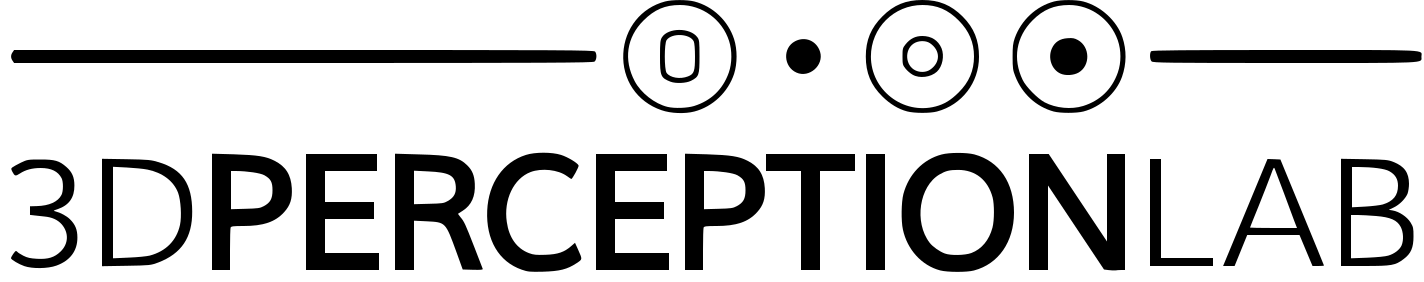
\includegraphics[height=0.7cm]{images/3dpl}
  \end{center}
\end{minipage}
}

% Clear the navigation bar
\setbeamertemplate{navigation symbols}{}
 
\subject{Sujet de la présentation}

\begin{document}

\begin{frame}
\titlepage
\end{frame}

\begin{frame}
  \frametitle{Table of Contents}
  \small
  \tableofcontents
  \normalsize
\end{frame}

\section{Introduction}
\label{sec:partie1}

\begin{frame}
  \frametitle{Introduction}
  \begin{center}
  	A visually realistic, flexible and robust grasping system for real-time interaction in Virtual Reality environments
  \end{center}
  	
  \begin{figure}
  	\centering
  	\includegraphics[width=0.9\textwidth]{images/intro}
  \end{figure}
\end{frame}

\begin{frame}
\frametitle{Introduction}
	\begin{itemize}
		\item VR objects extracted from the YCB dataset \cite{Calli2017}.
		\item Hands are controlled using handheld devices (e.g. Oculus Touch).
		\item Implemented in Unreal Engine 4.
		\item Qualitative analysis: 
		\begin{itemize}
			\item motor control.
			\item finger movement realism.
			\item interaction realism.
		\end{itemize}
		\item Quantitative analysis:
		\begin{itemize}
			\item novel metric quantifying hand-object overlapping.
			\item time needed to grasp each object.
		\end{itemize}
	\end{itemize}
\end{frame}

\section{Motivation}

\begin{frame}
\frametitle{Motivation}
\begin{itemize}
	\item Lack of realism of existing interactions in VR applications using handheld controllers.
	\begin{itemize}
		\item Distance-based grasping.
		\item Predefined grasp animations.
	\end{itemize}
	\item Lack of open-source approaches.
	\item Extract data from visually realistic interactions with everyday objects.
\end{itemize}

\begin{figure}
	\centering
	\includegraphics[width=0.7\textwidth]{images/grab}
	\caption{Distance grab example from Oculus Sample Framework \cite{oculusGrab}}
\end{figure}
\end{frame}


\section{Grasping System}

\begin{frame}
\frametitle{Grasping System}
The essence of our grasping system is how the hand is automatically fitted to the object shape. Our methodology consists of two main stages:
\begin{itemize}
	\item Virtual hand configuration:
	\begin{itemize}
		\item Choose the grasp animation according to a grasp taxonomy proposed by Feix et al. \cite{feix2016grasp}.
		\item Experimentally place the capsule triggers on the phalanges.
	\end{itemize}
	\item Grasping pipeline design and implementation.
\end{itemize}
\end{frame}


\begin{frame}
\frametitle{Grasping System- vr hand configuration}

\textbf{Choose the grasp animation}

\begin{itemize}
	\item We analyzed 33 different grasp types from the taxonomy.
	\item The cylindrical grasp:
	\begin{itemize}
		\item Power grasp.
		\item Palm opposition.
	\end{itemize}
\end{itemize}

\begin{figure}
	\centering
	\includegraphics[width=0.6\textwidth]{images/grasp_taxonomy}
	\caption{From left to right: pad, palm and side opposition.}
\end{figure}
\end{frame}


\begin{frame}
\frametitle{Grasping System- vr hand configuration}

\textbf{Triggers placement}

\begin{itemize}
	\item Progressively increase the number of capsules maintaining performance.
	\item Interact with small and different shaped objects using capsules only on the distal phalanges.
	\begin{itemize}
		\item Slippery behavior because of the collision with middle phalanges.
		\item \textbf{Solution:} put capsule triggers on the middle phalanges.
	\end{itemize}
	\item Put a sphere trigger on the hand palm to enable palm opposition.
\end{itemize}

\begin{figure}
	\centering
	\includegraphics[width=0.5\textwidth]{images/mannequin_hands}
	\caption{In green, capsule triggers of the middle and distal phalanges. In purple, sphere triggers used to detect the nearest object the the hand palm.}
\end{figure}
\end{frame}


\begin{frame}
\frametitle{Grasping System- pipeline}

\definecolor{lightgreen}{RGB}{166,196,138}
\definecolor{lightblue}{RGB}{143,184,237}

\tikzstyle{block} = [rectangle, draw, fill=lightgreen, 
text width=5em, text centered, rounded corners, minimum height=3em]
\tikzstyle{cloud} = [draw, ellipse, text centered, fill=lightblue, text width=4em,
minimum height=2em]
\tikzstyle{line} = [draw, -latex']

\begin{figure}[!t]
	\centering
	\resizebox{0.9\linewidth}{!}{
		\begin{tikzpicture}[node distance = 3cm, auto]
		% Place nodes
		\node [block] (init) {Object selection};
		\node [block, right of= init] (manager) {Interaction manager};
		\node [block, right of= manager] (movement) {Finger movement};
		\node [block, right of= movement] (logic) {Grasping logic};
		
		% Draw edges
		\path [line] (init) -- (manager);
		\path [line] (manager) -- (movement);
		\path [line] (movement) -- (logic);
		\end{tikzpicture}}$  $
	\label{fig:pipeline}
\end{figure}

\begin{itemize}
	\item Object selection: 
	\begin{itemize}
		\item selects the nearest object to the hand palm.
	\end{itemize}
	\item Interaction manager: 
	\begin{itemize}
		\item manages the capsule triggers placed on finger phalanges.
		\item determines phalanx state (blocked/released).	
	\end{itemize}
	\item Finger movement: 
	\begin{itemize}
		\item controls individual finger movement during interaction.
	\end{itemize}
	\item Grasping logic:
	\begin{itemize}
		\item decides when to grab or release an object.
	\end{itemize}
\end{itemize}

\end{frame}





\section{Performance analysis}

\begin{frame}
\frametitle{Performance analysis}

A qualitative evaluation:
\begin{itemize}
	\item based on: user experience interaction in a photorealistic environment.
	\item to assess: interaction realism, immersion, hand movement naturalness, etc.
\end{itemize}
A novel quantitative evaluation:
\begin{itemize}
	\item novel error metric.
	\item time needed to grasp the objects.
\end{itemize}

Two groups of users: experienced and inexperienced.


\end{frame}

\begin{frame}
	\frametitle{Performance analysis- dataset}
	
	\begin{figure}[!t]
		\centering
		\begin{subfigure}[t]{0.13\textwidth}
			\includegraphics[trim={9cm 1cm 8cm 6.3cm},clip,width=\textwidth]{../Figures/0.png}
			\caption{}
			\label{fig:masterchefcan}
		\end{subfigure}
		%add desired spacing between images, e. g. ~, \quad, \qquad, \hfill etc. 
		%(or a blank line to force the subfigure onto a new line)
		\begin{subfigure}[t]{0.13\textwidth}
			\includegraphics[trim={8cm 0cm 7cm 5cm},clip,width=\textwidth]{../Figures/1.png}
			\caption{}
			\label{fig:crackerbox}
		\end{subfigure}
		%add desired spacing between images, e. g. ~, \quad, \qquad, \hfill etc. 
		%(or a blank line to force the subfigure onto a new line)
		\begin{subfigure}[t]{0.13\textwidth}
			\includegraphics[trim={9cm 1.5cm 8.5cm 6.5cm},clip, width=\textwidth]{../Figures/2.png}
			\caption{}
			\label{fig:sugarbox}
		\end{subfigure}
		\begin{subfigure}[t]{0.13\textwidth}
			\includegraphics[trim={9.2cm 1.5cm 8.7cm 7cm},clip, width=\textwidth]{../Figures/3.png}
			\caption{}
			\label{fig:tomatosoupcan}
		\end{subfigure}
		\begin{subfigure}[t]{0.13\textwidth}
			\includegraphics[trim={8cm 1cm 8cm 5.5cm},clip, width=\textwidth]{../Figures/4.png}
			\caption{}
			\label{fig:mustardbottle}
		\end{subfigure}
		\begin{subfigure}[t]{0.13\textwidth}
			\includegraphics[trim={9cm 1.5cm 7cm 5cm},clip, width=\textwidth]{../Figures/5.png}
			\caption{}
			\label{fig:tunafishcan}
		\end{subfigure}
		\begin{subfigure}[t]{0.13\textwidth}
			\includegraphics[trim={9.5cm 1.5cm 7cm 5.5cm},clip, width=\textwidth]{../Figures/7.png}
			\caption{}
			\label{fig:gelatinbox}
		\end{subfigure}
		\centering
		\begin{subfigure}[t]{0.13\textwidth}
			\includegraphics[trim={8.5cm 0cm 7.5cm 7cm},clip, width=\textwidth]{../Figures/8.png}
			\caption{}
			\label{fig:pottedmeatcan}
		\end{subfigure}
		\begin{subfigure}[t]{0.13\textwidth}
			\includegraphics[trim={9cm 1cm 6cm 5cm},clip, width=\textwidth]{../Figures/9.png}
			\caption{}
			\label{fig:banana}
		\end{subfigure}
		\begin{subfigure}[t]{0.13\textwidth}
			\includegraphics[trim={10cm 2.5cm 7cm 5.5cm},clip, width=\textwidth]{../Figures/10.png}
			\caption{}
			\label{fig:strawberry}
		\end{subfigure}
		\begin{subfigure}[t]{0.13\textwidth}
			\includegraphics[trim={9.5cm 1.5cm 7cm 6cm},clip, width=\textwidth]{../Figures/11.png}
			\caption{}
			\label{fig:apple}
		\end{subfigure}
		\begin{subfigure}[t]{0.13\textwidth}
			\includegraphics[trim={10cm 1.5cm 7cm 6.5cm},clip, width=\textwidth]{../Figures/12.png}
			\caption{}
			\label{fig:lemon}
		\end{subfigure}
		\begin{subfigure}[t]{0.13\textwidth}
			\includegraphics[trim={9.5cm 2.08cm 8cm 6cm},clip, width=\textwidth]{../Figures/13.png}
			\caption{}
			\label{fig:peach}
		\end{subfigure}
		\begin{subfigure}[t]{0.13\textwidth}
			\includegraphics[trim={9.5cm 2.3cm 7.5cm 5.2cm},clip, width=\textwidth]{../Figures/14.png}
			\caption{}
			\label{fig:pear}
		\end{subfigure}
		\begin{subfigure}[t]{0.13\textwidth}
			\includegraphics[trim={9.7cm 2cm 8cm 6.3cm},clip, width=\textwidth]{../Figures/15.png}
			\caption{}
			\label{fig:orange}
		\end{subfigure}
		\begin{subfigure}[t]{0.13\textwidth}
			\includegraphics[trim={9.5cm 2cm 7cm 5.5cm},clip, width=\textwidth]{../Figures/16.png}
			\caption{}
			\label{fig:plum}
		\end{subfigure}
		\begin{subfigure}[t]{0.13\textwidth}
			\includegraphics[trim={7cm 1cm 7cm 4cm},clip, width=\textwidth]{../Figures/17.png}
			\caption{}
			\label{fig:bleachcleaner}
		\end{subfigure}
		\begin{subfigure}[t]{0.13\textwidth}
			\includegraphics[trim={8cm 2cm 6cm 5cm},clip, width=\textwidth]{../Figures/18.png}
			\caption{}
			\label{fig:fork}
		\end{subfigure}
		\begin{subfigure}[t]{0.13\textwidth}
			\includegraphics[trim={9cm 1.8cm 6cm 6cm},clip, width=\textwidth]{../Figures/19.png}
			\caption{}
			\label{fig:spoon}
		\end{subfigure}
		\begin{subfigure}[t]{0.13\textwidth}
			\includegraphics[trim={9cm 4.2cm 6cm 3.5cm},clip, width=\textwidth]{../Figures/20.png}
			\caption{}
			\label{fig:knife}
		\end{subfigure}
		\begin{subfigure}[t]{0.13\textwidth}
			\includegraphics[trim={8cm 2cm 6cm 5cm},clip, width=\textwidth]{../Figures/21.png}
			\caption{}
			\label{fig:spatula}
		\end{subfigure}
	\end{figure}
	
\end{frame}

\begin{frame}
	\frametitle{Performance analysis- dataset}
	
	\begin{figure}[!t]
		\begin{subfigure}[t]{0.13\textwidth}
			\includegraphics[trim={7cm 1cm 7cm 5cm},clip, width=\textwidth]{../Figures/22.png}
			\caption{}
			\label{fig:powerdrill}
		\end{subfigure}
		\begin{subfigure}[t]{0.13\textwidth}
			\includegraphics[trim={8cm 3cm 7cm 5cm},clip, width=\textwidth]{../Figures/23.png}
			\caption{}
			\label{fig:scissors}
		\end{subfigure}
		\begin{subfigure}[t]{0.13\textwidth}
			\includegraphics[trim={10cm 3cm 8cm 5.5cm},clip, width=\textwidth]{../Figures/24.png}
			\caption{}
			\label{fig:largemarker}
		\end{subfigure}
		\begin{subfigure}[t]{0.13\textwidth}
			\includegraphics[trim={9cm 2cm 7cm 4cm},clip, width=\textwidth]{../Figures/25.png}
			\caption{}
			\label{fig:adjustablewrench}
		\end{subfigure}
		\begin{subfigure}[t]{0.13\textwidth}
			\includegraphics[trim={7.5cm 2cm 8cm 4.5cm},clip, width=\textwidth]{../Figures/27.png}
			\caption{}
			\label{fig:flatscrewdriver}
		\end{subfigure}
		\begin{subfigure}[t]{0.13\textwidth}
			\includegraphics[trim={7cm 0.8cm 6cm 3cm},clip, width=\textwidth]{../Figures/28.png}
			\caption{}
			\label{fig:hammer}
		\end{subfigure}
		\begin{subfigure}[t]{0.13\textwidth}
			\includegraphics[trim={10cm 2.5cm 7cm 5.5cm},clip, width=\textwidth]{../Figures/29.png}
			\caption{}
			\label{fig:baseball}
		\end{subfigure}
		\begin{subfigure}[t]{0.13\textwidth}
			\includegraphics[trim={9.5cm 2cm 7cm 5.5cm},clip, width=\textwidth]{../Figures/30.png}
			\caption{}
			\label{fig:tennisball}
		\end{subfigure}
		\begin{subfigure}[t]{0.13\textwidth}
			\includegraphics[trim={6cm 1.5cm 7cm 4cm},clip, width=\textwidth]{../Figures/34.png}
			\caption{}
			\label{fig:toyairplane}
		\end{subfigure}
		\caption{Grasping performed on objects from the YCB dataset.}\label{fig:ycbgrasps}
	\end{figure}
	
\end{frame}



\begin{frame}
	\frametitle{Performance analysis- qualitative}
	
	\begin{table}[!t]
		\resizebox{\linewidth}{!}{
			\begin{tabular}{cl}
				\hline
				\textbf{ID} & \textbf{Question}\\
				\hline
				\multicolumn{2}{c}{\emph{Aspect 1: Motor Control}}\\
				Q1 & I felt like I could control the virtual hands as if it were my own hands\\
				Q2 & The movements of the virtual hands were caused by my movements\\
				Q3 & I felt as if the movements of the virtual hands were influencing my own movements\\
				Q4 & I felt as if the virtual hands were moving by themselves\\
				\hline
				\multicolumn{2}{c}{\emph{Aspect 2: Finger Movement Realism}}\\
				\hline
				Q5 & It seemed that finger movements were smooth and plausible\\
				Q6 & I felt fingers open and close in a natural way\\
				Q7 & Fingers react adequately to my intentions\\
				\hline
				\multicolumn{2}{c}{\emph{Aspect 3: Interaction Realism}}\\
				\hline
				Q8 & I felt like I could grab objects wherever I wanted to\\
				Q9 & It seemed as if the virtual fingers were mine when grabbing an object\\
				Q10 & I felt that grabbing objects was clumsy and hard to achieve\\
				Q11 & It seemed as if finger movement were guided and unnatural\\
				Q12 & I felt that grasps were visually correct and natural\\
				Q13 & I felt that grasps were physically correct and natural\\
				Q14 & It seemed that fingers were adapting properly to the different geometries\\
				\hline
		\end{tabular}}
		\caption{User evaluation questionnaire.}
		\label{table:questionnaire}
	\end{table}
	
	
\end{frame}

\begin{frame}
	\frametitle{Performance analysis- qualitative}
	
	\begin{table}[!t]
		\resizebox{0.95\linewidth}{!}{
			\begin{tabular}{lcc}
				\hline
				& \multicolumn{2}{c}{Score} \\
				\cline{2-3}
				Evaluation Aspects    & Experienced users & Inexperienced users \\
				\hline
				(1) Motor Control     & 1.85    & 2.34      \\
				(2) Finger Movement Realism & 2.33   & 2.51       \\
				(3) Interaction Realism      & 1.84     & 1.95      \\
				\hline
				Embodiment score & 1.97 &  2.19 \\
				\hline
		\end{tabular}}
		\caption{Score for each qualitative aspect of the evaluation and group of participants.}
		\label{table:qualitativeresults}
	\end{table}
	
	\begin{itemize}
		\item 7-point Likert-scale [-3,3].
		\item Average result of 2.08.
	\end{itemize}
\end{frame}




\begin{frame}
\frametitle{Performance analysis- quantitative}

\begin{figure}
	\centering
	\includegraphics[width=0.8\textwidth]{images/distanceCalculusMod}
\end{figure}


\end{frame}


\begin{frame}
\frametitle{Performance analysis- quantitative}

\begin{center}
	\begin{adjustbox}{width=\textwidth}
		\begin{tikzpicture}
		\begin{axis}[
		ybar= 0pt,
		xtick=data,
		symbolic x coords= {a,b,c,d,e,f,g,h,i,j,k,l,m,n,o,p,q,r,s,t,u,v,w,x,y,z,aa,ab,ac,ad},
		x tick label style={anchor=north},
		typeset ticklabels with strut,
		enlarge x limits=0.025,
		enlarge y limits=0.3,
		bar width=0.38 em,
		grid=both,
		grid style={line width=.1pt, draw=gray!10},
		major grid style={line width=.2pt,draw=gray!50},
		ylabel={Time [$s$]},
		xlabel={Object [$id$]},
		width=1.3\textwidth,
		height=6cm,
		legend style={legend cell align=left, align=left, draw=white!15!black, legend columns= -1},
		legend pos=north west
		]
		\addplot[azure, fill=azure!40] table[x=object,y=0]{Data/time_per_object.dat};
		\addplot[red, fill=red!40] table[x=object,y=1]{Data/time_per_object.dat};
		%\addplot[green, fill=green!40] table[x=object,y=0]{Data/time_per_object_overall.dat};
		\legend{Experienced users, Inexperienced users}
		\end{axis}
		\end{tikzpicture}
	\end{adjustbox}
	%\caption{Average time (top) needed to grasp each object and average error (bottom) of the performed grasps.}
	%\label{chart:timeanderror}
\end{center}

\begin{itemize}
	\item Inexperienced users have taken longer to grasp the objects. 
	\item More time is needed because of random spawn.
\end{itemize}	

\end{frame}

\begin{frame}
\frametitle{Performance analysis- quantitative}

\begin{center}
	\begin{adjustbox}{width=\textwidth}
		\begin{tikzpicture}
		\begin{axis}[
		ybar= 0pt,
		xtick=data,
		symbolic x coords= {a,b,c,d,e,f,g,h,i,j,k,l,m,n,o,p,q,r,s,t,u,v,w,x,y,z,aa,ab,ac,ad},
		x tick label style={anchor=north},
		typeset ticklabels with strut,
		enlarge x limits=0.025,
		enlarge y limits=0.3,
		bar width=0.5 em,
		grid=both,
		grid style={line width=.1pt, draw=gray!10},
		major grid style={line width=.2pt,draw=gray!50},
		ylabel={Time [$s$]},
		xlabel={Object [$id$]},
		width=1.3\textwidth,
		height=6cm,
		legend style={legend cell align=left, align=left, draw=white!15!black, legend columns= -1},
		legend pos=north west
		]
		%\addplot[azure, fill=azure!40] table[x=object,y=0]{Data/time_per_object.dat};
		%\addplot[red, fill=red!40] table[x=object,y=1]{Data/time_per_object.dat};
		\addplot[green, fill=green!40] table[x=object,y=0]{Data/time_per_object_overall.dat};
		\legend{All users}
		\end{axis}
		\end{tikzpicture}
	\end{adjustbox}
	%\caption{Average time (top) needed to grasp each object and average error (bottom) of the performed grasps.}
	%\label{chart:timeanderror}
\end{center}

\begin{itemize}
	\item Larger objects are more time consuming.
	\item Less time is needed as the user gains experience.
\end{itemize}
\end{frame}


\begin{frame}
\frametitle{Performance analysis- quantitative}

\begin{center}
	\begin{adjustbox}{width=\textwidth}
		\begin{tikzpicture}
		\begin{axis}[
		ybar= 0pt,
		xtick=data,
		symbolic x coords= {a,b,c,d,e,f,g,h,i,j,k,l,m,n,o,p,q,r,s,t,u,v,w,x,y,z,aa,ab,ac,ad},
		x tick label style={anchor=north},
		typeset ticklabels with strut,
		enlarge x limits=0.025,
		enlarge y limits=0.05,
		bar width=0.38 em,
		grid=both,
		grid style={line width=.1pt, draw=gray!10},
		major grid style={line width=.2pt,draw=gray!50},
		ylabel={Error [$mm$]},
		xlabel={Object [$id$]},
		width=1.3\textwidth,
		height=6cm,
		legend style={legend cell align=left, align=left, draw=white!15!black, legend columns= -1},
		legend pos=north west
		]
		\addplot[azure, fill=azure!40] table[x=object,y=0]{Data/accuracy_per_object.dat};
		\addplot[red, fill=red!40] table[x=object,y=1]{Data/accuracy_per_object.dat};
		%\addplot[green, fill=green!40] table[x=object,y=0]{Data/time_per_object_overall.dat};
		\legend{Experienced users, Inexperienced users}
		\end{axis}
		\end{tikzpicture}
	\end{adjustbox}
\end{center}

\begin{itemize}
	\item Similar results regardless of previous VR experience.
	\item Most differences: power drill (u) and spatula (v).
\end{itemize}

\end{frame}


\begin{frame}
\frametitle{Performance analysis- quantitative}

\begin{center}
	\begin{adjustbox}{width=\textwidth}
		\begin{tikzpicture}
		\begin{axis}[
		ybar= 0pt,
		xtick=data,
		symbolic x coords= {a,b,c,d,e,f,g,h,i,j,k,l,m,n,o,p,q,r,s,t,u,v,w,x,y,z,aa,ab,ac,ad},
		x tick label style={anchor=north},
		typeset ticklabels with strut,
		enlarge x limits=0.025,
		enlarge y limits=0.05,
		bar width=0.38 em,
		grid=both,
		grid style={line width=.1pt, draw=gray!10},
		major grid style={line width=.2pt,draw=gray!50},
		ylabel={Error [$mm$]},
		xlabel={Object [$id$]},
		width=1.3\textwidth,
		height=6cm,
		legend style={legend cell align=left, align=left, draw=white!15!black, legend columns= -1},
		legend pos=north west
		]
		%\addplot[azure, fill=azure!40] table[x=object,y=0]{Data/accuracy_per_object.dat};
		%\addplot[red, fill=red!40] table[x=object,y=1]{Data/accuracy_per_object.dat};
		\addplot[green, fill=green!40] table[x=object,y=0]{Data/time_per_object_overall.dat};
		\legend{All users}
		\end{axis}
		\end{tikzpicture}
	\end{adjustbox}
\end{center}

\begin{itemize}
	\item Large objects are the most error-prone.
	\item Overall error is decreasing progressively.
\end{itemize}

\end{frame}



\section{Applications}

\begin{frame}
	\frametitle{Applications}

\begin{itemize}
	\item Robotics: human-robot knowledge transfer.
	\item Rehabilitation: patients with hand motor difficulties.
	\item Data generation.
\end{itemize}	

\end{frame}

\section{Limitations and future works}

\begin{frame}
	\frametitle{Limitations and future works}
	
	\begin{itemize}
		\item Single animation for hand closing.
		\item Cannot grasp one object with both hands at the same time.
		\item Interaction with large objects require VR skills.
	\end{itemize}
\end{frame}

\section{Conclusions}

\begin{frame}
	\frametitle{Conclusions}
	
	\begin{itemize}
		\item We proposed a grasping system for interaction in VR where hand is automatically fitted to the object geometry.
		\item We analyzed our proposal both qualitatively and quantitatively.
		\item For the quantitative evaluation we proposed a novel metric quantifying the hand-object overlapping at the distal and middle phalanges.
		\item Performance analysis results indicate that previous experience with our grasping system is not a prerequisite for an enjoyable VR interaction experience.
	\end{itemize}
	
\end{frame}


\begin{frame}
	\titlepage
\end{frame}


\newcounter{lastframe}
\setcounter{lastframe}{\insertframenumber}

\begin{frame}[allowframebreaks]{References}
\bibliographystyle{authoryear-fr}
\bibliography{references}
\end{frame}

\setcounter{framenumber}{\thelastframe}

\begin{frame}
	\frametitle{Grasping System- pipeline}
	
	\textbf{Grasping logic}
	
	\begin{equation} \label{eq:3}
	f(th_{ph}, in_{ph}, mi_{ph}, palm)= 
	\begin{cases}
	true, & \text{if } (th_{ph} \lor palm) \\
	& \land (in_{ph} \lor mi_{ph})\\
	false,              & \text{otherwise}
	\end{cases}
	\end{equation}, where $th_{ph}$, $in_{ph}$, and $mi_{ph}$ are defined as
	
	\begin{equation} \label{eq:4}
	\begin{array}{l}
	th_{ph} = thumb_{mid} \lor thumb_{dist} \\
	in_{ph} = index_{mid} \lor index_{dist} \\
	mi_{ph} = middle_{mid} \lor middle_{dist} \\
	\end{array}
	\end{equation}
	
\end{frame}

\begin{frame}
	\frametitle{Performance analysis- qualitative}
	
	
	\begin{equation}\label{eq:6}
	\begin{split}
	\text{Motor Control} &= ((Q1 + Q2) - (Q3 + Q4)) / 4 \\
	\text{Finger Movement Realism} &= (Q5 + Q6 + Q7) / 3 \\
	\text{Interaction Realism} &= ((Q8 + Q9) - (Q10 + Q11)\\
	& + Q12 + Q13 + Q14) / 7 
	\end{split}
	\end{equation}, using the results of each individual aspect, we obtain the total embodiment score as follows:
	\begin{equation} \label{eq:5}
	\begin{split}
	\text{Score} &= (\text{Motor Control} + \text{Finger Movement Realism} \\
	& + \text{Interaction Realism} * 2) / 4
	\end{split}
	\end{equation}
	
\end{frame}

\end{document}
